\documentclass[english]{cgspaper} % change option to 'english' to include english logo in \copyrightspace

%\usepackage[ngerman]{babel} % comment out to use english in auto-generated section titles
\usepackage[utf8]{inputenc}
\usepackage[ruled]{algorithm}
\usepackage{algpseudocode}
\usepackage{url}
\usepackage{csquotes}

\title{Demonstration of Game-Based Object Detection}
\author{Tom Beckmann\\ Digital Engineering Faculty, Hasso Plattner Institute \textbar{} University of Potsdam}
\author{Philipp Bode\\ Digital Engineering Faculty, Hasso Plattner Institute \textbar{} University of Potsdam}
\author{Julius C. R. Rudolph\\ Digital Engineering Faculty, Hasso Plattner Institute \textbar{} University of Potsdam}
\author{Hendrik Rätz\\ Digital Engineering Faculty, Hasso Plattner Institute \textbar{} University of Potsdam}

% Konfiguration des Veranstaltungs-Feldes
\subject{%
    \textbf{Advanced Games of Life}\\
    Sommersemester 2018\\
    Themenstellung und Anleitung:
    Daniel Limberger und Prof.\ Dr.\ Jürgen Döllner}

\begin{document}

% Definition des Teasers
\teaser{
    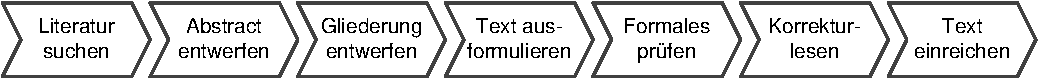
\includegraphics[width=0.9\textwidth]{graphics/prozess.pdf}
    \caption{Beispiel für einen Teaser: Schritte beim Erstellen eines fachwissenschaftlichen Beitrags. Ein Teaser dient als Blickfang schon auf der ersten Seite eines Artikels.}
    \label{fig:prozess}
}

\maketitle

%----------------------------------------------------------------
% Zusammenfassung
%----------------------------------------------------------------
\begin{abstract}
\end{abstract}

\copyrightspace % Erzeugt den Hinweis auf die Veranstaltung links unten
%----------------------------------------------------------------
% Introduction
%----------------------------------------------------------------
\section{Introduction}
- features of today's smartphones 
 - cameras able to take high resolution pictures/videos
 - geolocation via GPS
 - ability to use high speed internet (where available) -> send high amounts of data/video streaming possible
 - high processing power, multiple cores, quite some RAM
 - allows complex calculations, analysis of video data, e.g. in context of AR

- Pokemon-Go
- popular game about catching Pokemon in the real world
- around 800 million downloads (30.5.18, https://www.playm.de/2018/05/pokemon-go-35-403807/)

- uses location of user to identify Pokemon/Events/special places near him
- able to use AR to interact with Pokemon in real world 
- (always) connected to the internet and able to transfer data, no opt-out

- possible to create very detailed profiles of players
- tracking of location and movement (further analysis could discover certain habits/patterns)
- analysis of everything where persons points their camera at: texts, faces, brands
- can be used for espionage, preparation of crimes or simply targeted advertisements

- hence we created a demo showcase to reveal the potential dangers that the improvident usage of AR-apps can bring

%----------------------------------------------------------------
% Lehrstuhlkontext: 
% Diesen Abschnitt (in der deutschen bzw. englischen Fassung) übernehmen 
%----------------------------------------------------------------

%\section{Kontext}
%\label{sec:Kontext}
%Die Betreuung im Rahmen der Seminartätigkeit erfolgte durch das Fachgebiet für Computergrafische Systeme, dessen Forschungsschwerpunkt die Prozessierung, Abbildung und interaktive Visualisierung massiver raumzeitlicher \cite{Oehlke2015,Buschmann2015,Buschmann2014,Maass2006} sowie abstrakter, hochdimensionaler Daten \cite{Limberger2017,Limberger2016,Wuerfel2015} ist. Dies beinhaltet neben neuartigen Algorithmen \cite{RichterKyprianidis2013,RichterBehrens2013,Glander2012}, Rendering-Techniken \cite{Semmo2016,Pasewaldt2014,Maass2006a,Doellner2005} und Interaktions-Metaphern \cite{Semmo2016a,Scheibel2016,Semmo2014} auch effiziente Datenstrukturen \cite{Scheibel2017,Richter2015} und Systemarchitekturen \cite{Klimke2014,Trapp2012,Klimke2010}, die anhand von real-weltlicher Datensätze und Anwendungsszenarien  \cite{Discher2016,Trapp2015,Engel2012} evaluiert werden. 

\section{Context}
\label{sec:Context}
This course project was supervised by the Computer Graphics Systems Group whose main research interest includes the processing, mapping, and interactive visualization of massive spatio-temporal information \cite{Oehlke2015,Buschmann2015,Buschmann2014,Maass2006} and abstract high-dimensional information \cite{Limberger2017,Limberger2016,Wuerfel2015}. In particular, this comprises novel algorithms \cite{RichterKyprianidis2013,RichterBehrens2013,Glander2012}, rendering techniques \cite{Semmo2016,Pasewaldt2014,Maass2006a,Doellner2005}, and interaction metaphors \cite{Semmo2016a,Scheibel2016,Semmo2014}, as well as efficient data structures \cite{Scheibel2017,Richter2015} and system architectures \cite{Klimke2014,Trapp2012,Klimke2010} which are evaluated based on real-world data sets and application scenarios \cite{Discher2016,Trapp2015,Engel2012}.


%----------------------------------------------------------------
% Related Work
%----------------------------------------------------------------
\section{Related Work}
\label{sec:related_work}
Related projects/Work

% Wie analysieren wir diese?

%----------------------------------------------------------------
% Concept
%----------------------------------------------------------------
\section{Privacy intrusion through AR and CV technologies}

-(factor 1) Advancement of augmented reality technologies (robustness, accuracy) and ease of integration (AR libraries) will presumably lead to a surge in mobile applications utilizing such features. \\
-(factor 2) Current AR applications are often developed for entertainment purposes or as feature showcase, but with increasing maturity of the technology, conceivable use cases appear in a wide range of domains, e.g. information display in professional environments, medical application, support of sensory functions, etc. \\
- (factor 3) By necessity, AR applications are granted permission to access the camera input of the mobile device. This opens up a visual window into the immediate and intimate vicinity of the user, often in their homes or work places. \\
- Additionally, advancements in computer vision increase the computational interpretability of pictures or even extensive near real time analysis of video feeds.

-> \textbf{Large scale data mining of the user's analog environment becomes  conceivable.}

- Malicious actor: Could uncover sensitive information that is heavily protected in the digital world.
Possible desirable information could be tax identification numbers, bank account numbers, social security numbers, etc., i.e. anything that can often be found in plain sight on sensitive documents but is well-encrypted in digital representations.

-Authoritarian governments: Surveillance use cases; automatic detection of contraband or illicit material, even cues for dissident tendencies. Potential for integration of analysis capabilities on the OS level with e.g. a custom Android distribution.

- Profit driven actor: Allows the creation of precise consumer profiles for targeted advertising and audience selection. Could provide insights that classical profiles generated by online behaviour analysis lack.

However, mere panning over a room's interior does not provide images with a high enough resolution to gather most often fine-printed information.
Techniques like optical character recognition (OCR) that enable the automatic processing of captured text require close-ups shots of points of interest.
With the Demon Go prototype, we try to lead the user into providing these necessary close-up shots.
In order to hide the video analysis from the user, we align the requirements on the camera feed with plausible and engaging game mechanics.

\section{Game Concept}
\label{sec:concept}

% - premise: camera is able to generate lots of (sensitive) data
% - challenge: camera is not always focused on points of interest
% - use case if solved: points where interesting information about user can be seen/user which can be used for espionage, commercial use, etc.
% - solution: guide user to move camera/focus on PoI through gameplay elements



% Concept
- 4 elements: gathering energy points (the in-game currency), capturing demons, beat other players in combat, beat their demons protecting the stashes

- main goal for the player is to "dominate" as much of the real world as possible

%- Therefore it's necessary that the player places stashes at fixed geo-locations whose range of influence can be extended by placing demons on them which furthermore defend the stashes against attackers 
%- (for implementation: the stronger the demons, the bigger the range of influence --> direct correlation) 
%- stashes can only be placed at current location

%- in the area of influence of one player it's not possible for other players to place their stashes --> hence players are forced to attack hostile stashes to decrease their area of influence (by killing defending demons) or ideally to destroy the whole stash and steal in-game currency called energy/experience points placed by the defender

\subsection{Getting Demons}
\label{subsec:demons}

- with the virtual currency the user is able to summon new demons that can then be used to fight other stashes or to defend the own stashes

- for summoning the user needs to be in the area of influence of one of his stashes --> the bigger and stronger the stash, the higher the likelihood of a successful incantation (or a stronger demon)
--> this makes it very likely for the user to place a stash somewhere where he often goes to 
--> assumption: users will defend their real world homes, work places, schools, universities, ... to increase their time to summon demons

- another way to collect demons is to catch demons which are present in the real world
- therefore an AR view is used in which the user has to find, follow, fight and finally catch the demons
- scan room with phone if demon is close and combat it in order to catch it
- demon is trying to avoid capture by flying around while player is trying to weaken it by shooting (tapping demon on screen) it and, once the demon is "weakened", casting spells to bind it (drawing special figures on screen)
- on success demon is captured by player and will be added to the user's demon collection. from there it can be user to attack other stashes, to defend own stashes or to sacrifice it to receive EP for it

\subsection{Stashes and EP}
\label{subsec:stashesandep}

- not possible to "carry" unlimited amount of EP 
- stashes serve as deposit boxes for EP

- stashes mark territory of player (circle around stash)
- can only be placed at current location
- are visible to all other players 
- have to be defended against attackers
- range of influence can be extended by placing demons on them which furthermore defend the stashes against attackers 
- also the max capacity of EP that the stash can hold increases with the strength of the defending demons

- in the area of influence of one player it's not possible for other players to place their stashes --> hence players are forced to attack hostile stashes to decrease their area of influence (by killing defending demons) or ideally to destroy the whole stash and steal in-game currency called energy/experience points placed by the defender

- forces players to place stashes in the real world 
- provokes other players to limit their possible range of influence and steal the stashed EPs
--> are player's game progress
--> should be hard to destroy

- multiple stati

1. created stash with no EP in it --> only visible to creator as long as no demons and no EPs in it

2. when EP deposited but no demon placed to defend --> visible to everyone with blue perimeter, showing that EP are free to collect for everyone in a specific range (currently 100 m)

3. when alive demons are defending it --> red perimeter for opponent stashes, yellow for own stashes. perimeter range depending on strength of defending demons
--> player cannot see defending demons of hostile stashes --> makes it more unpredictable how good stashes are defended
- also allows for "bluffs" (player can place many demons on a stash without having any EP in it) e.g. just to restrict/narrow the max area of other players

%- stashes are visible to other players (on the map) and can be attacked by them (currently only one demon at the time) 

\subsection{Attacking and defending stashes}
\label{subsec:attackingstashes}

- players can attack stashes of others

- battling stashes (currently) always involves exactly two parties, an attacking demon and a static collection of defending demons which were placed on the attacked stash in advance

- when attacker wins the fight the EP of the defeated stash get exposed 
- is shown to everyone and everyone nearby can collect the EP by clicking on the stash (if he has enough capacity) --> currently user needs to be in a radius of 100 m around the stash 

--> motivates players to move irl and to expose more documents/sensitive content

- also motivates other players to check regularly if they have a defeated stash nearby to collect the EP

[picture of defeated stash]

- the fights are conceptualized that it's hard to destroy a stash as stashes and the deposited EP within them are basically the user's game progress
- and as one stash can theoretically be attacked by everyone

- nevertheless opponent players obviously have the chance to ally to pursue their common goal of decreasing a strong defender's range of influence (currently need to communicate irl, later possibly in app)

- very important to balance the summoning cost of different kinds of demons with the possible amount of EP an attacker can receive when destroying a stash
- hasn't been tested with real users for the current implementation

\subsection{Future Gameplay Ideas}
\label{subsec:futuregameplayideas}

- when player attacks a stash: demon first has to get to the stash --> dependant on the distance to stash 

- show the attacking demon on map next to the defenders and display current fight status over their icons

%- as stashes are publicly visible to everyone and as stashes and the deposited EP within them are basically the user's game progress it was necessary to make it hard for attackers to destroy a stash

- [include pictures of every step]

\subsection{Collecting Data}
\label{subsec:collectingdata}

% Welche Daten sammeln wir dabei? → “Dämon als Datenpunkt”
- capturing a demon: two phases
- phase 1: scanning, demon is flying around randomly while the captured camera frames are processed
- camera frames are rated by specific metrics. goal is to identify interesting points (e.g. text, brands, faces) to send the user to -> best frames are PoI
- phase 2: capturing, demon flies to PoI to force the user to point camera at it and "cast the spell" (i.e. hold phone relatively even while pointing at the PoI and with half of the view covered by pattern/finger)
- more detailed processing of captured frames
(- also geolocation of user can be captured when he places stashes/moves around to attack others)

% Berechtigungen ergeben Sinn
- principle to not fabricate the threat too much:
- all permissions which the user has to grant are used in the game and their use is easily comprehensible for the user
 - Camera: AR
 - Location: place and attack stashes available at real world locations
 - Internet: Needed to sync with other players, get information about demons
 
% Möglichst geringe Ressourcennutzung
- not possible to stream all frames to server for further analysis -> would use too much bandwidth
- also processing of every single frame on the server would take too much time 
- preprocess frames and rate them -> only send best frames to server


%----------------------------------------------------------------
% Implementation
%----------------------------------------------------------------

% Implementierung des Spielkonzepts (vermutlich mit Fokus auf AR)
% Limitierungen von AR (bzw. Wie gehen wir damit um?)

\section{Gameplay Implementation}
\label{sec:gameplay_implementation}
- game uses AR to capture demons; involves getting idea about the location, correlating it to 2d frames that are analyzed by pipeline

\subsection{ARCore}
- ARCore: definition, scope of the library, other applications (FIXME: move to a background section?)
- Concepts: session w/ tracking info, anchors, plane detection --> focused on getting a stable "game board"

- our use: getting an idea about the room's dimensions, moving objects in virtual scene believably relative to phone's movement
- estimating room size: incentivizing turning by defining a "start room" for demon that progressively grows --> assumes user is not pressed against a wall
- problems w/ room size: abusing tracking points might include outliers that artificially extend the room --> makes game elements inaccessible; fast movement may reduce quality

\subsection{Map View}
- using MapBox to display an interactive map of the augmented world with markers at the positions of stashes (different colors for own and hostile stashes) with their perimeter/range of influence
- for own stashes the user also sees icons for every demon he placed to defend the stash 

- markers are pinned by geo-location on the map

\subsection{Storing and syncing stash data}
- need to easily sync the current game state (players, stashes, demons) across multiple clients on different devices

- using document-based NoSQL-database Google Firestore (cloud hosting, synced state across clients, easy setup) --> current flagship database of Google for mobile app development

- document hierarchy: player id --> stashes/null stash --> demons for stash (everything indexed by id)

- App implements change listeners for the collections of stashes and demons --> depending on what type of event happened stash/demon markers on the map (ideally only nearby) need to be redrawn
--> updated after every fight and every placement of a demon onto a stash

- demons that the player didn't place at a stash are saved in the player's "null-stash" which is not saved in the collection of stashes (as it does not need to be synced with the other players)
- updated when new demon was summoned or captured and after every fight in which the attacking demon lost health points

\subsection{Demon fights}

- the current implementation is a simulation that follows a round-based approach. In every round the attacking demon assaults one defending demon and afterwards gets assaulted by every defending demon sequentially. Thereby both the order in which the defenders are attacked by the attacker and the order in which the defenders counter-attack the attacking demon are shuffled once in advance of the fight. 

- makes the fight more unpredictable and harder for the attacker to guess which demons he might eliminate. After a fight both users are informed about the result (using Android Toast/Push Notification) and the health points of the surviving demons are updated in the corresponding Google Firestore documents.

- as users can currently add an unlimited amount of demons to a stash the defense of a stash gets exponentially stronger the more demons the defender places on them

- in a future version: defender can interactively intervene in the fight and dynamically add more defenders to the stash -> therefore fight must obviously take a while


\subsection{Snapshots}
- every frame is distilled into a "Snapshot" containing pixel data, all tracking points, view-proj-matrices. pixel data is passed on to pipeline
- pipeline reports back with 2d PoI
- challenge: likely won't have depth component for an arbitrary point on image
- solution: project tracking points to 2d plane, find closest

- pipeline calls project method, stores best hits for PoI
- game/AR component later requests best 0-5 PoI from pipeline
- generates random ones within room at reachable height to make game experience more consistent (i.e. not make game easier in plain rooms)

\section{Data Analysis Implementation}
\begin{figure*}
    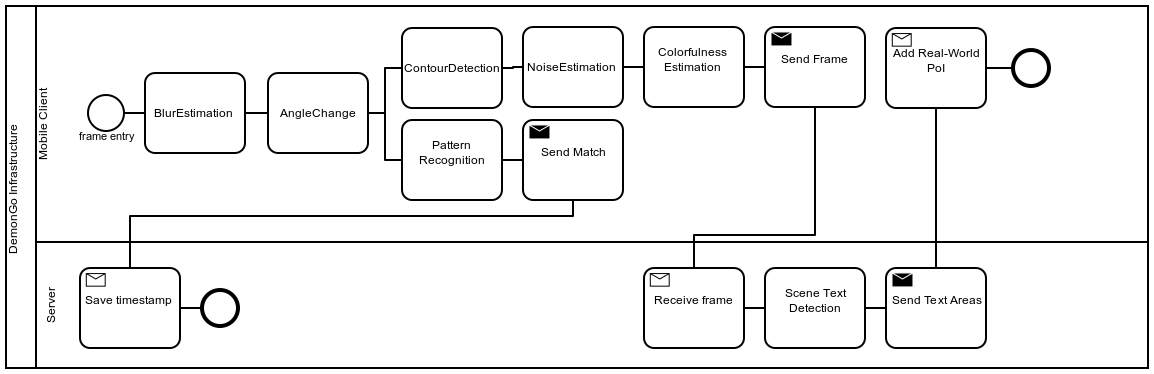
\includegraphics[width=\textwidth]{graphics/pipeline_phase_1.png}
    \caption{Pipeline Phase 1}
    \label{fig:prozess}
\end{figure*}

% FIXME intro to OpenCV, features, usages?
- pipeline which processes every frame (captured by camera while capturing demons) on phone
- preselect frames which are sent to server
- only best should get sent
- pipeline consists of independent sets which could be ordered in any order -> same interface
- frames are wrapped in \textit{Snapshots} (ensures that the same object is passed between steps)

\subsection{Snapshots / Communication with Pipeline}
% FIXME in parts dupl with ARCore.Snapshots above -- might be fine if we focus on the pipeline-specific aspects
- holds OpenCV Mat (represents frame) and score (calculated in steps)
- also able to convert Mat to base64 and make a parameter list out of attributes (both for sending) 

- AR-Snapshots: additional fields (points in room and viewProjectionMatrix)

\subsection{Steps}
- contain list of following steps (in next)
- able to track time of execution
- .start(snap) -> .process(snap) -> .output(snap) (starts all steps in next with processed snapshots)

- special case: \textit{StepWithQueue}
- additional priority queue based on snapshot score
- getBestAndClear (angleChange) and getBest (sendingStep)
- used in angleChange and sendingStep where the only the best frame should be handled/should be handled first

% Daten-Analyse-Pipeline
 % Finden von PoI
 % Capturing und Processing
 
 \subsubsection{Blur Estimation}
 - try to use/analyze only those frames which are not too blurry and send those to the server (reduce traffic)
 - convert image to grayscale (only one channel)
 - apply Laplace Operator (edge detection)
 - calculate variance of it 
 -> used as score for blurriness: low value = high blurriness, high value = low blurriness
 - reason: Laplace detects edges, if edges are not to clear (low variance) picture may be blurry
 - transform blurriness value to value between 0 and 1 (everything above 500 is 1 everything else bluriness value/500)
\subsubsection{Brand/Pattern Recognition}
- Utilizes keypoint detection and feature descriptor matching to match recognizable patterns like brand logos and letterings \\
- The ORB (Oriented FAST and Rotated BRIEF) technique is used \cite{rublee2011orb} \\
- Computationally expensive step is keypoint calculation for frame.\\
-> Comparison with large number of patterns possible, as their keypoints can be precalculated.

\subsubsection{Contour Detection}
- Gaussian Blur -> bilateral filter -> Canny edge detection -> find Contours and cull by minimum size and maximal edges.\\
- Found contours are cropped and passed to next steps for likelihood of text estimation

\subsubsection{Noise Estimation}
- A simple kernel for fast noise estimation for which the authors note \enquote{In textured images or regions, though, the noise estimator perceives thin lines as noise.} \cite{immerkaer1996fast}. \\
- We utilize this property to detect probable regions with dense text.

\subsubsection{Colorfulness Estimation}
- Simple measure for estimating colorfulness of an image \cite{hasler2003measuring}. \\
- We presume that regions of legible text are usually low in color variance to increase the contrast between letters and background.

\subsection{Communication between phone and server}
- uses volley to send POST-requests to server
- adds best captured frame (out of Snapshot queue) to Volley-request-queue every 0.5s
- base64 encoded frame
- also adds a unique user ID and firebase token to request
- sending of requests in background asap

- every 100th frame is put directly into sending queue after going through blurriness and anglechange
- if no/few frames make it through the rest of the pipeline (contourdetction/noise) at least some frame frames are getting sent to server
- if over frames are in sending queue, frames with better scores are transmitted first


\subsection{Server-side Analysis}

- Flask/Flask-SocketIO server with sqllite db
- decodes received images and writes them to the disk (for now)
- detects where possible text is written on saved image
- crops image for every box \& saves it
- analyses rotaion of text, removes rotation and runs pytesseract on it 
- saves user\_id, filename of cropped img, analysed text, rotation, timestamp and confidence of analysis (given by pytesseract) to db
- also informs the frontend (?) about added and processed images via SocketIO


%----------------------------------------------------------------
% Evaluation
%----------------------------------------------------------------

\section{Evaluation}
\label{sec:evaluation}

% AR-Komponente (Bewegung des Dämons, Werden die PoI’s wiedergefunden, etc.)
- biggest challenge: ensuring that tracking points at PoI remain consistent as user approaches; old visual context is lost as they focus e.g. on a single part of the desktop --> might cause ARCore to recalc coordinate system (could have been nice to pause allocation of tracking points and rely on accelerometer, but ARCore does not support this)
% FIXME: to be tested further:
- by defining anchors on the relevant tracking points, ARCore will ensure most of the time that objects remain within reach -- timeout and fallback to showing spell even though user is not close enough otherwise

- movement of demon feels weird at start, as dimensions of room are unknown
- placement of waypoints close to user confuse, but as they traverse the room and turn frequently it's hard to predict where they will be

% FIXME: to be evaluated if that applies to anyone else but me:
- handling of phone is tricky: most users held phone in right hand, shot w/ left hand in scanning phase. switch hands when entering capturing phase for drawing spells --> messes up coordinate system as phone points to floor temporarily

% Erkennung der Points of Interest
- Blurriness: Laplacian is not too precise, e.g. when using shallow focus, some regions are completely focused whereas some are totally blurry
--> will result in low blurriness value

% Brand-Detection

% Textanalyse mit OCR
- Wo wird im Bild Text erkannt?
- Kann dieser Text interpretiert werden, wenn ja, wie gut?
- Was sind Probleme? (Schriftart, Blurriness, distortion)

% Scalability

%----------------------------------------------------------------
% Conclusion
%----------------------------------------------------------------
\section{Conclusion}
\label{sec:conclusion}

% Future Work
- z.B. weitere Daten sammeln und komplexere Nutzerprofile anlegen
- Data Analytics auf den gesammelten Infos

%----------------------------------------------------------------
% Sources
%----------------------------------------------------------------
\bibliographystyle{acmsiggraph}
\bibliography{foo-paper}

\end{document}
